\documentclass{article}

% Language setting
% Replace `english' with e.g. `spanish' to change the document language
\usepackage[english]{babel}

% Set page size and margins
% Replace `letterpaper' with `a4paper' for UK/EU standard size
\usepackage[letterpaper,top=2cm,bottom=2cm,left=3cm,right=3cm,marginparwidth=1.75cm]{geometry}
\usepackage{bm}

% Useful packages
\usepackage{amsmath}
\usepackage{amssymb}

\usepackage{algorithm}
\usepackage{algpseudocode}
\usepackage{appendix}

\usepackage{graphicx}
\usepackage[colorlinks=true, allcolors=blue]{hyperref}

\usepackage{subcaption}

\usepackage{tikz}

% Costume Style Begin
\usepackage{enumitem}

\usepackage{listings}
\usepackage{xcolor}

\lstset{
    language=Python,
    basicstyle=\ttfamily\small,
    keywordstyle=\color{blue},
    commentstyle=\color{green!60!black},
    stringstyle=\color{red},
    tabsize=4,
    showspaces=false,
    showstringspaces=false,
    frame=single,
}
% Costume Style End

% Operator Declaration Begin

% Operator Declaration End

\title{SUSTech CS324 2024 Spring Assignment 2 Report}
\author{12110304 Chunhui XU}

\begin{document}
\maketitle

\section{Part 1 Task 1 \& 2}

\subsection{Simple Introduction}

In these tasks, I need to create a simple MLP by \texttt{PyTorch}. And compare the training situation with the realization by \texttt{NumPy}.

The MLP structure just as which in Assignment 1, and I'll compare \texttt{torch} and \texttt{numpy} implementation in \texttt{make\_moon} and two other datasets.

\subsection{\texttt{torch} Feature Analysis}

In torch, we could use the pre-defined utils.

For exmaple: common layers, such as linear layer and ReLU layer, can simply use \texttt{nn.Linear} and \texttt{nn.ReLU}, they have there own \texttt{forward()} functions. Once they are initialization with \texttt{nn.Sequential()}, we can directly get output from input by passing it through each layer one by one.

Use \texttt{nn.CrossEntropyLoss()} to compute the Cross Entropy loss of the model. Through \texttt{torch.optim}, we can adjust parameters in layers, implement backward propagation.

\subsection{Global Settings}

\subsubsection{Default Parameters}

\begin{itemize}
    \item \texttt{dnn\_hidden\_units}: $[20]$, comma separated list of number of units in each hidden layer
    \item \texttt{learning\_rate}: $1\mathrm{e}^{-2}$, learning rate for optimization
    \item \texttt{max\_steps}: $1500$, number of steps to run trainer
    \item \texttt{eval\_freq}: $10$, frequency of evaluation on the test set
    \item \texttt{batch\_size}: $800$, batch size of single train batch
\end{itemize}

\subsubsection{MLP Structure}

\begin{enumerate}
    \item $2$ input
    \item $2 \to 20$ Linear Layer
    \item $20 \to 20$ ReLU Layer
    \item $20 \to 2$ Linear Layer
    \item $2 \to 2$ Softmax Layer
    \item One hot output and Cross Entropy loss function
    \item Gradient descent strategy: BGD idea actually, refer to \ref{sec:p1t1_ana_loss}.
\end{enumerate}

\subsubsection{Dataset Generation}

I use code to visually demonstrate the generation method of the dataset.

\begin{lstlisting}[language=Python]
from sklearn.preprocessing import OneHotEncoder
from sklearn.datasets import *

x, y = [], [] # input and label
if type_id == 1:
    self.type_name = 'moon'
    x, y = make_moons(n_samples=1000, noise=0.05)
elif type_id == 2:
    self.type_name = 'blobs'
    x, y = make_blobs(n_samples=1000, centers=2, cluster_std=3)
elif type_id == 3:
    self.type_name = 'gaussian_quantiles'
    x, y = make_gaussian_quantiles(n_samples=1000, n_classes=2)
y = OneHotEncoder(sparse_output=False).fit_transform(y.reshape(-1, 1))
\end{lstlisting}

\subsection{Result Visualization}

There are 3 figures, fig \ref{fig:p1t1_moon} for \texttt{make\_moon}, fig \ref{fig:p1t1_blobs} for \texttt{make\_blobs}, fig \ref{fig:p1t1_gaussian_quantiles} for \texttt{make\_gaussian\_quantiles},

\begin{figure}[!htp]
  \centering
  \begin{subfigure}[b]{0.85\textwidth}
    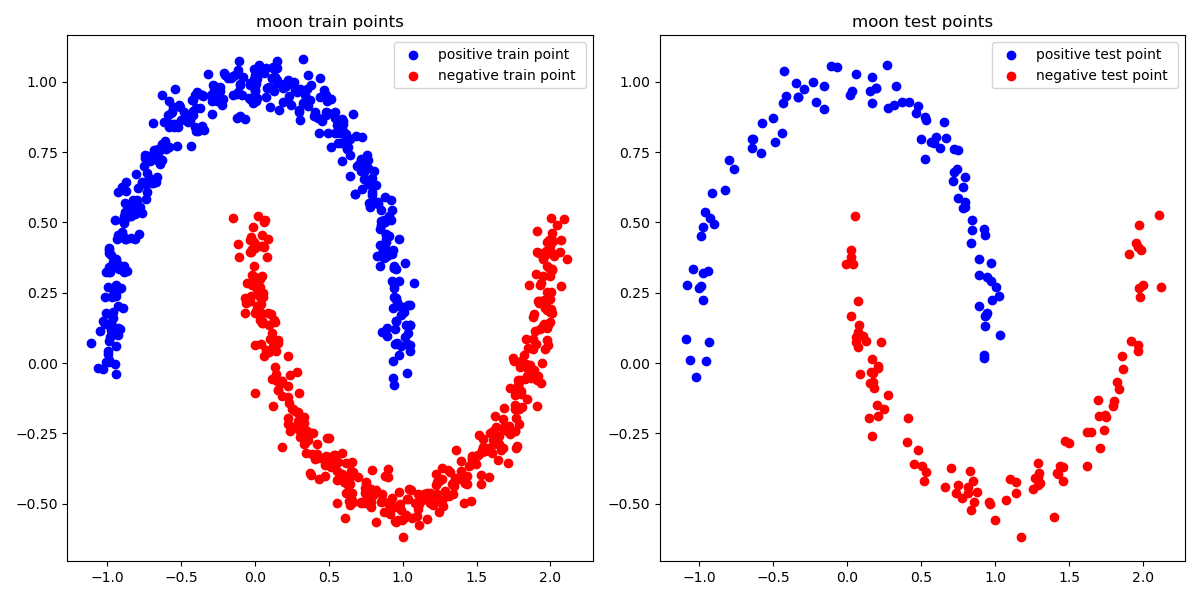
\includegraphics[width=\textwidth]{img/Part1/data_moon.png}
    \caption{Blobs Data}
  \end{subfigure}
  \begin{subfigure}[b]{0.9\textwidth}
    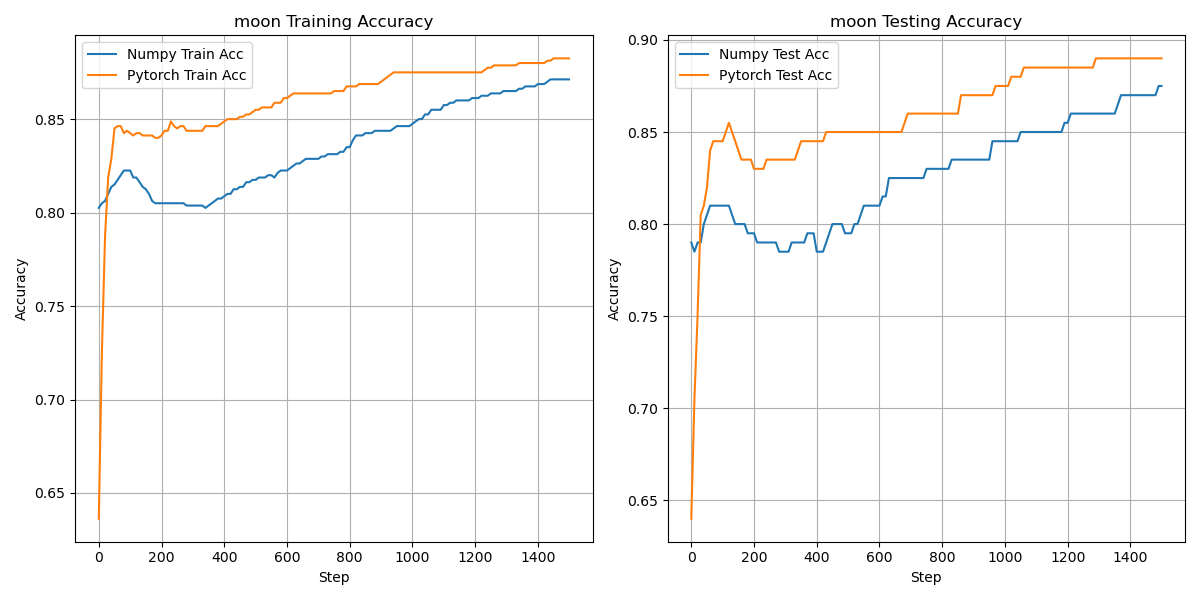
\includegraphics[width=\textwidth]{img/Part1/acc_moon.png}
    \caption{Blobs Accuracy}
  \end{subfigure}
\begin{subfigure}[b]{0.9\textwidth}
    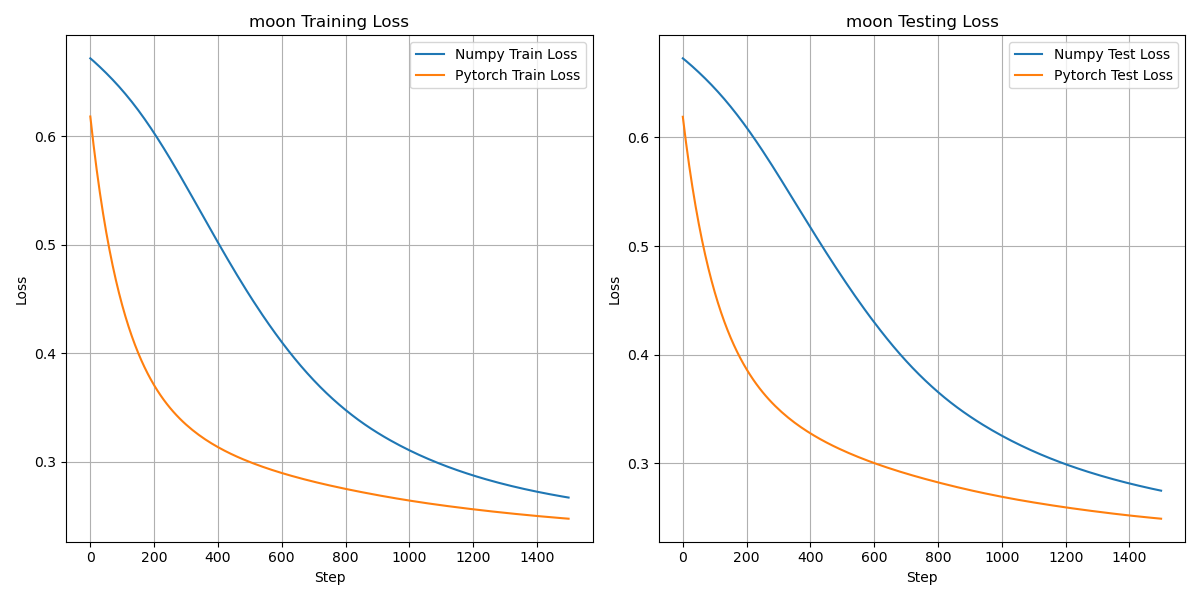
\includegraphics[width=\textwidth]{img/Part1/loss_moon.png}
    \caption{Blobs Loss}
  \end{subfigure}
  \caption{Blobs numpy \& torch}
  \label{fig:p1t1_moon}
\end{figure}

\subsection{Result Analysis}

\subsubsection{Overall Analysis}

Through different images for several different datasets, it can be observed that despite the different implementation approaches of the two models, as long as the model architecture remains constant, their characteristic curves exhibit similarities, both in terms of accuracy and loss. This mutual approve both of my implementations within this simple MLP structure are reasonable.

\subsubsection{Dataset Analysis}

Simple analysis: The model has different performance in three data sets: the data set of blobs is widely separated, and it is easy to achieve high performance; moon is second. For gaussian quantiles, intuitively speaking, the data distribution of it cannot be divided by a simple decision boundary, and accordingly the accuracy increases relatively slowly with training.

\subsubsection{Loss Analysis}\label{sec:p1t1_ana_loss}

Although I utilized \texttt{optim.SGD()} as the optimizer, I actually realize the BGD. I did not perform any data splitting during input; instead, I fed all inputs as a whole to the MLP for computation. Therefore, in practice, what I achieved was finding the global optimum through gradient descent, which is the concept of Batch Gradient Descent (BGD). From this, it can be inferred that the descent of the training loss curve is smooth, devoid of any fluctuations.

\section{Part 1 Task 3}

\subsection{Global Settings}

\subsubsection{Default Parameters}

\begin{itemize}
    \item \texttt{dnn\_hidden\_units}: $[512, 64]$, comma separated list of number of units in each hidden layer
    \item \texttt{learning\_rate}: $1\mathrm{e}^{-3}$, learning rate for optimization
    \item \texttt{max\_epochs}: $150$, number of steps to run trainer
    \item \texttt{eval\_freq}: $1$, frequency of evaluation on the test set
    \item \texttt{batch\_size}: $32$, batch size of single train batch
\end{itemize}

\subsubsection{MLP Structure}

\begin{enumerate}
    \item $3 \times 32 \times 32$ input
    \item $3072 \to 512 $ Linear Layer    
    \item $512 \to 512 $ ReLU Layer
    \item $512 \to 64 $ Linear Layer
    \item $64 \to 64 $ ReLU Layer
    \item $64 \to 10 $ Linear Layer
    \item $10 \to 10$ Softmax Layer
    \item $10$ output
\end{enumerate}

\subsection{Result Visualization}

Fig \ref{fig:p1t3_cifar_adam} show the accuracy and loss in CIFAR-10 dataset with Adam optimizer, while fig \ref{fig:p1t3_cifar_sgd} is SGD.

\begin{figure}[!htbp]
    \centering
    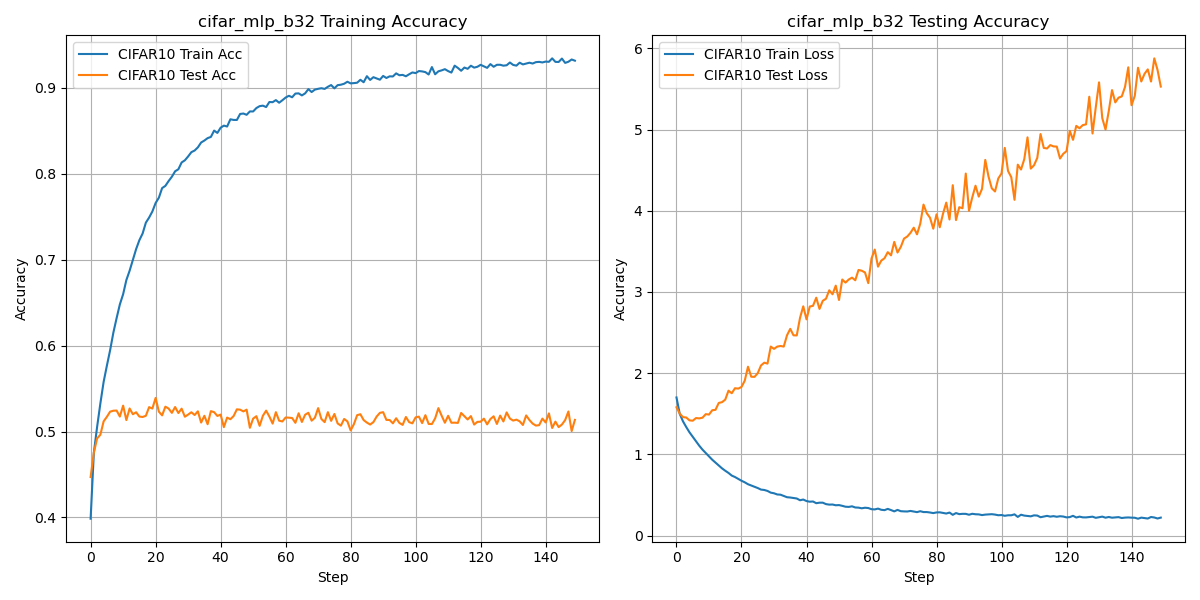
\includegraphics[width=1\textwidth]{img/Part1/cifar_mlp_b32_adam.png}
    \caption{MLP CIFAR-10 Curve}
    \label{fig:p1t3_cifar_adam}
\end{figure}


\subsection{Result Analysis}

\subsubsection{MLP Analysis}

In the MLP, I choose $3 \times 32 \times 32$ as input. Because for CIFAR-10 picture, it has $32 \times 32$ as the pixel width and height. In the picture, each pixel has red, green, blue 3 channels. Therefore, I got the $3072$ feature inputs.

In hidden layer, I set two hidden layers, there size is 512, 64. As a simple dataset, I don't want to add too complex hidden layers for MLP, so I choose these hidden layer size.

Finally, I got output of size 10, indicating the possibility of each class in CIFAR-10, and I choose the max one as the final classification result.

\subsubsection{Feature Analysis}

Overall, we can find a very interesting situation: as the number of training times continues to increase, the accuracy of the training set quickly reached 90\%, while the accuracy of the test set stagnated at 50\% after a brief rise. Finally, it has been unable to rise. And by carefully observing the Loss curve, we will also find an additional fact: the Loss of the test set is even rising!

This leads to an obvious concept: overfitting. With continuous training, MLP overfits the training data, and its parameters are constantly customized according to the training data, but it loses generalization and cannot well extract some general features in the CIFAR-10 data set.

So why is there such a big deviation in the performance of MLP on CIFAR-10 compared to the classification problem of Assignment1? Here are a few possible reasons I guess:

\begin{itemize}
    \item \textbf{Fully connected features}: MLP is a fully connected structure, which means that everything in the image data will affect the final result. The image data may contain edges, interference, and other data that are not helpful or even disruptive to the analysis results, thus causing a lot of problems in the MLP learning process and overfitting.
    \item \textbf{The structure of hidden layers is too simple}: I only set up two hidden layers [512, 64]. Such a simple structure cannot extract the deep features of the image well, which leads to a decrease in the generalization ability of the model and leads to overfitting.
\end{itemize}

In short, although MLP classification was tried on CIFAR-10, due to some objective limitations, its actual effect was not very satisfactory. In the Part 2, I will try to use CNN to complete the CIFAR-10 image classification problem.

\section{Part 2 Task 1}

\subsection{Simple Introduction}

In this task, I need to create a simple CNN. The structure is listed in lecture slide. I analyze the layers feature and compute the input and output shape in this part.

\subsection{CNN Structure}

The structure Defined by lecture slide, fig \ref{fig:p2_cnn_structure}:

For pooling layer, $k$ stand for kernel size, $s$ stand for stride, $p$ stand for padding.

\begin{figure}[!htbp]
    \centering
    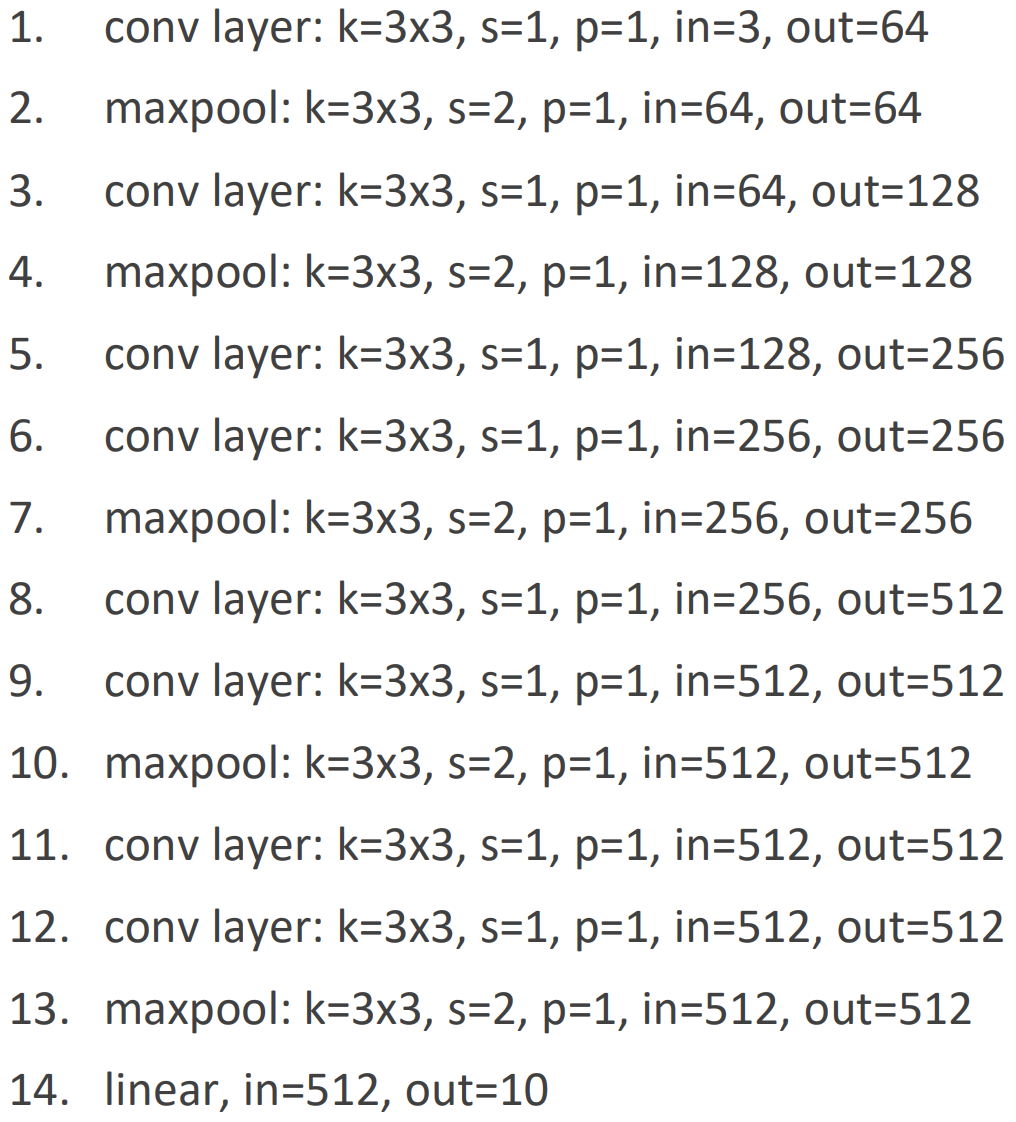
\includegraphics[width=0.5\textwidth]{img/Part2/CNN_structure.png}
    \caption{CNN Structure Detail}
    \label{fig:p2_cnn_structure}
\end{figure}

\subsection{Input Output Size}

\begin{itemize}
    \item The convolution layer change the channel number.

    \item {
        The height and width computation for pooling layer is:

        $$ H_{out} = \left\lfloor \frac{H_{in} - k_{h} + 2 \times p}{s} \right\rfloor + 1 $$
        
        $$ W_{out} = \left\lfloor \frac{W_{in} - k_{w} + 2 \times p}{s} \right\rfloor + 1 $$
        }
        
    \item The ReLU layer does not change the shape of  data.
\end{itemize}

And table \ref{tab:network_layers} shows the final output for each layer which change the data shape:

\begin{table}[!ht]
\centering\caption{Output of each layer in CNN}
\label{tab:network_layers}
\begin{tabular}{|c|c|}
\hline
\textbf{Layer} & \textbf{Output Size} \\
\hline
Conv2d & $32 \times 32 \times 64$ \\ \hline
MaxPool & $16 \times 16 \times 64$ \\ \hline
Conv2d & $16 \times 16 \times 128$ \\ \hline
MaxPool & $8 \times 8 \times 128$ \\ \hline
Conv2d & $8 \times 8 \times 256$ \\ \hline
Conv2d & $8 \times 8 \times 256$ \\ \hline
MaxPool & $4 \times 4 \times 256$ \\ \hline
Conv2d & $4 \times 4 \times 512$ \\ \hline
Conv2d & $4 \times 4 \times 512$ \\ \hline
MaxPool & $2 \times 2 \times 512$ \\ \hline
Conv2d & $2 \times 2 \times 512$ \\ \hline
Conv2d & $2 \times 2 \times 512$ \\ \hline
MaxPool & $1 \times 1 \times 512$ \\ \hline
Flatten & $512$ \\ \hline
Linear & $10$ \\ \hline
\end{tabular}
\end{table}

\section{Part 2 Task 2}

\subsection{Simple Introduction}

In this part, I will train my CNN on CIFAR-10 dataset with default parameters, and compare the different result with changing parameters following the single variable principle.

\subsection{Default Parameters}

\begin{itemize}
    \item \texttt{optimizer\_type}: 'ADAM' (indicating \texttt{torch.optim.Adam}), type of optimizer for the model training
    \item \texttt{learning\_rate}: $1\mathrm{e}^{-4}$, learning rate for optimization
    \item \texttt{max\_epochs}: $200$, number of epochs to run trainer
    \item \texttt{eval\_freq}: $1$, frequency of evaluation on the test set
    \item \texttt{batch\_size}: $32$, batch size of single train batch
\end{itemize}

\subsection{Result Visualization}

Actually, in the beginning of this part, I train $1000+$ epochs to get the result. But I found that the training accuracy will converge after $200$ epochs. So follow TA’s explanation, I use $200$ epoch for the rest to get results faster.

Table \ref{tab:p2_res_para} shows different parameters and corresponding figure.

\begin{table}[!h]
\centering\caption{Different Parameters and Result}
\label{tab:p2_res_para}
\begin{tabular}{|c|c|}
\hline
\textbf{Fig ID} & \textbf{Single Variable Content} \\
\hline
Fig \ref{fig:p2_default} & Default Parameters \\ \hline
Fig \ref{fig:p2_sgd} & Change optimizer to \texttt{torch.optim.SGD} \\ \hline
Fig \ref{fig:p2_RMS} & Change optimizer to \texttt{torch.optim.RMSprop} \\ \hline
Fig \ref{fig:p2_lr_1e-3} & Change learning rate to $1\mathrm{e}^{-3}$ \\ \hline
Fig \ref{fig:p2_lr_5e-2} & Change learning rate to $5\mathrm{e}^{-2}$ \\ \hline
\end{tabular}
\end{table}

\begin{figure}[!htp]
  \centering
  \begin{subfigure}[b]{1\textwidth}
    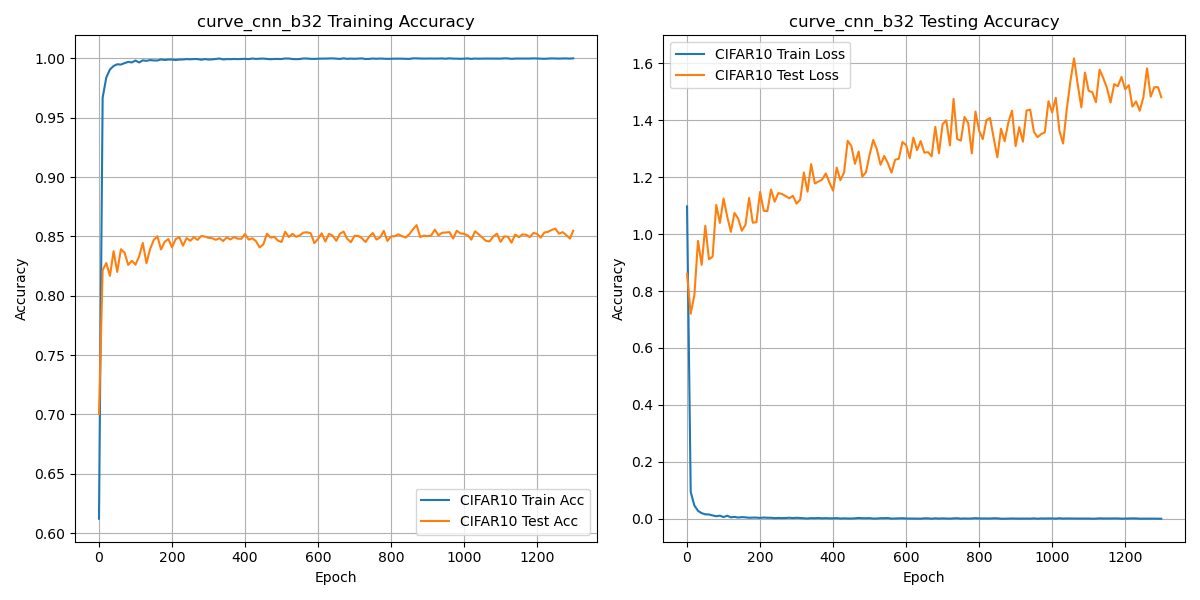
\includegraphics[width=\textwidth]{img/Part2/curve_cnn_default.png}
    \caption{Accuracy and Loss}
  \end{subfigure}
  \begin{subfigure}[b]{1\textwidth}
    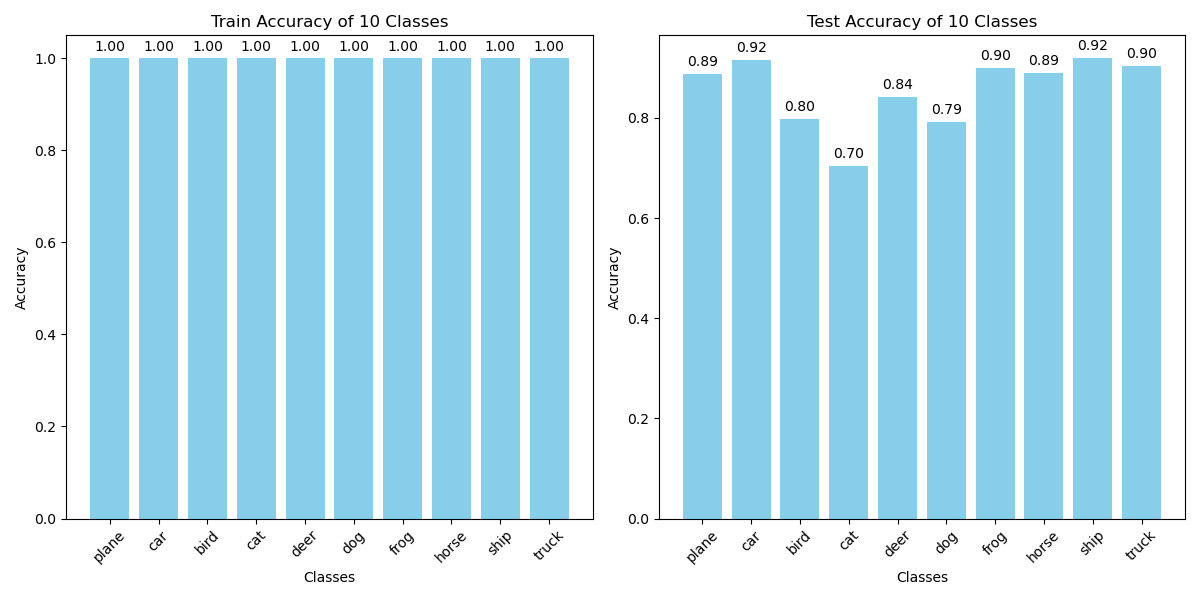
\includegraphics[width=\textwidth]{img/Part2/acc_cnn_class_default.png}
    \caption{Class Accuracy}
  \end{subfigure}
  \caption{Default Parameters}
  \label{fig:p2_default}
\end{figure}

\subsection{Result Analysis}

\subsubsection{Overall Analysis}

In the following sections, unless specified, the accuracy refers to the test accuracy by default.

Comparing with MLP, we can clearly find that the test accuracy of CNN has been significantly improved. Not only has the accuracy of the training set increased rapidly, but more importantly, the accuracy of the test set has been significantly improved, with the highest level staying at around 85\%. This directly shows that compared to MLP, CNN has made very significant progress on the CIFAR-10 data set, or by extension, the task of image classification.

However, by observing the curve, we can easily find that CNN cannot get rid of the problem of over-fitting. As the number of training increases, after a brief decline, the test loss slowly rises. In fact, through training with default parameters, it can be found that this increase still exists after $1000+$ epochs.

In general, CNN still has its limitations. If we want to achieve better accuracy, more appropriate structures and better optimization strategies are needed.

\subsubsection{Optimizer Analysis}

In the comparison of optimizers, I found that Adam, RMSprop, as an optimizer, has a very good learning effect, and the accuracy within the specified $200$ epochs can reach 85\% in the end; in contrast, the final accuracy of SGD is lower. Only at 78-80\%.

After search the information, I found that the biggest difference is that both Adam and RMSprop use adaptive learning rate optimization algorithms and can dynamically adjust the learning rate. Such dynamic adjustment can not only ensure the efficiency of back propagation updates, but also prevent it from falling into the trap of local optimality like SGD.

Among them, Adam adjusts the learning rate for each parameter based on the first and second moment estimates (mean and variance) of its gradient. And RMSprop adjusts the learning rate using the moving average of squared gradients, it uses the exponential decay average of squared gradients.

In image classification, a task with deeper networks, an optimizer with more strategies and an adaptive learning rate is more suitable. If we really want to find the advantages of SGD, it may be the train speed is slightly faster.

\subsubsection{Class Accuracy Analysis}

Through the type accuracy I output, we can also find interesting phenomena: the overall classification accuracy of car, ship, truck, etc. is significantly higher, while the overall classification accuracy of dog, cat, bird, etc. is lower.

We can make a bold guess: there are some similarities between animals, and cats and dogs themselves are especially similar. In contrast, frog, as an amphibian, does not seem to be similar so much.

Therefore, we can see that in image classification tasks, our human intuitive feelings are also has hidden relationship with the feature of the data itself.

\subsubsection{Learning Rate Analysis}

Comparing the learning rates, we can see that appropriately increasing the learning rate ($1\mathrm{e}^{-3}$) can improve learning efficiency and speed up convergence (even with the assistance of Adam Optimizer). However, an inappropriately large learning rate ($5\mathrm{e}^{-2}$) makes the upper limit of accuracy convergence lower, and the curve oscillates very violently. The step when adjusting the parameters each time is too large, resulting in continuous missing of the extreme value, and only keeps oscillating near the extreme value, making it impossible to get close.

This is why in practical deep learning, the learning rate should not be too large.

\section{Part 3 Task 1}

\subsection{Simple Introduction}

In this task, I need to create a simple RNN following the given formula. I shall realize the RNN without \texttt{torch.nn.RNN} or \texttt{torch.nn.LSTM}

\subsection{Structure Analyze}

\subsubsection{RNN Modules}

The requirement give series formula:

\begin{align}
    h^{(t)} &= \tanh{(W_{hx}x^{(t)} + W_{hh}h^{(t-1)} + b_h)} \label{eq:rnn_main} \\ 
    o^{(t)} &= (W_{ph}h^{(t)} + b_o) \label{eq:rnn_ouput_layer} \\ 
    {\tilde{y}^{(t)}} &= \text{softmax}(o^{(t)}) \label{eq:rnn_softmax}
\end{align}

According to these formula, I create 3 linear layer to realize the whole RNN operations:

\begin{lstlisting}[language=Python]
    # w_hx * xt + bh
    self.hx = nn.Linear(input_dim, hidden_dim, bias=True)
    # w_hh * h_(t-1)
    self.hh = nn.Linear(hidden_dim, hidden_dim, bias=False)
    # o_t = w_ph * h_t + b_o
    self.ho = nn.Linear(hidden_dim, output_dim, bias=True)
\end{lstlisting}

And I will explain the function of them:

\begin{enumerate}
    \item hx: $1 \to 128$. Linear Layer with bias, implement equation \ref{eq:rnn_main} $x^{(t)}$ part, let new input digit to hidden layer size.
    \item hh: $128 \to 128$. Linear Layer without bias, implement equation \ref{eq:rnn_main} $h^{(t-1)}$ part, let last time $h$ output get a weight in computation of new $h$.
    \item ho: $128 \to 10$. Linear Layer with bias, implement equation \ref{eq:rnn_ouput_layer}. Get the final predicted number from $[0, 9]$.
    \item a softmax layer, implement equation \ref{eq:rnn_softmax}
\end{enumerate}

\subsubsection{Forward Propagation}

When doing forward propagation:

\begin{lstlisting}[language=Python]
def forward(self, x):
    batch_size, input_length = x.size(0), x.size(1)
    h_last = torch.zeros(batch_size, self.hidden_dim).to(self.device)
    for t in range(input_length):
        x_cur = x[:, t, :]
        h_last = torch.tanh(self.hx(x_cur) + self.hh(h_last))
    out = self.softmax(self.ho(h_last))
    return out
\end{lstlisting}

I use a \texttt{for} loop to let the $x$ and previous $h$ participant the computation together, implement the RNN computation. And finally get the output.

After forward propagation, let the max value of the $10$ dimension item become the prediction result. 

\section{Part 3 Task 2}

\subsection{Simple Introduction}

In this part, I will train my RNN on palindrome dataset with input length $4$ and $19$, and let the RNN predict the last number of the palindrome number.

\subsection{Default Parameters}


\begin{itemize}
    \item \texttt{input\_length}: $19$, length of input sequence
    \item \texttt{input\_dim}: $1$, dimension of input data
    \item \texttt{num\_classes}: $10$, number of classes in the classification task
    \item \texttt{num\_hidden}: $128$, number of hidden units in the neural network
    \item \texttt{batch\_size}: $128$, batch size for training
    \item \texttt{learning\_rate}: $0.001$, learning rate for optimization
    \item \texttt{max\_epoch}: $1000$, maximum number of epochs to train the model
    \item \texttt{max\_norm}: $10$, maximum norm constraint for gradient clipping
    \item \texttt{data\_size}: $1000000$, size of the dataset
    \item \texttt{portion\_train}: $0.8$, portion of the dataset used for training
\end{itemize}

And I use \texttt{torch.optim.lr\_scheduler.StepLR()} (and step\_size=10, gamma=0.7) for scheduler,  but it has some interesting unexpected influence. Let me analysis it in the following part.

\subsection{Result Visualization}

Fig \ref{fig:p3_t=5} show a $T=5$ for RNN training, while fig \ref{fig:p3_t=20} show a $T=20$.

\begin{figure}[!htbp]
  \centering
  \begin{subfigure}[b]{1\textwidth}
    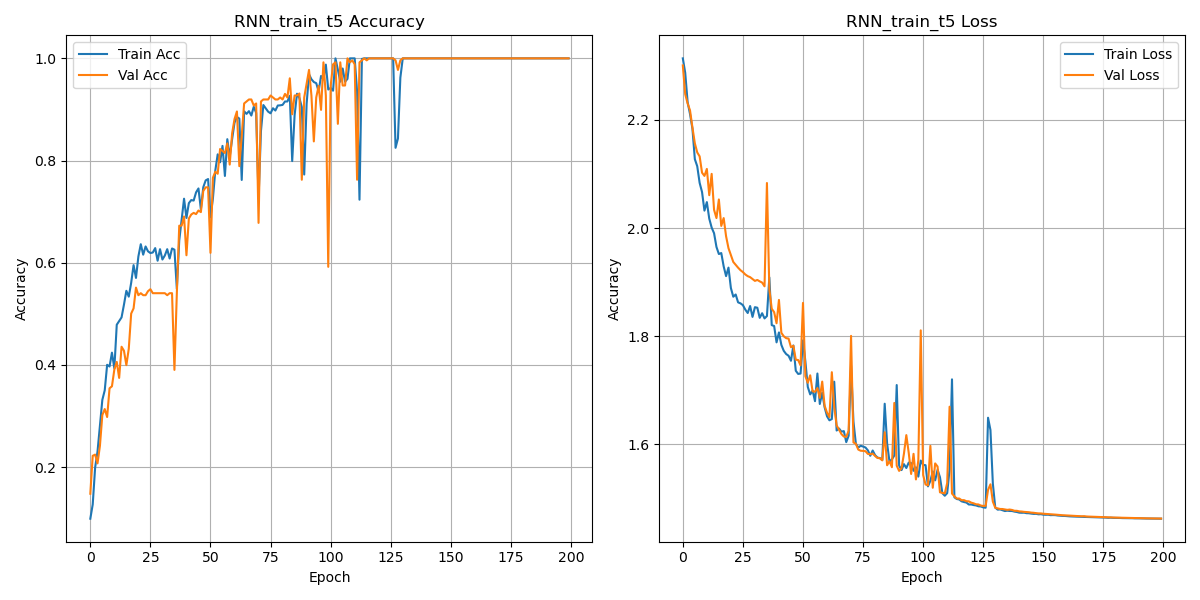
\includegraphics[width=\textwidth]{img/Part3/RNN_train_t5.png}
    \caption{$T=5$ Normal Curve (without scheduler)}
  \end{subfigure}
  \begin{subfigure}[b]{1\textwidth}
    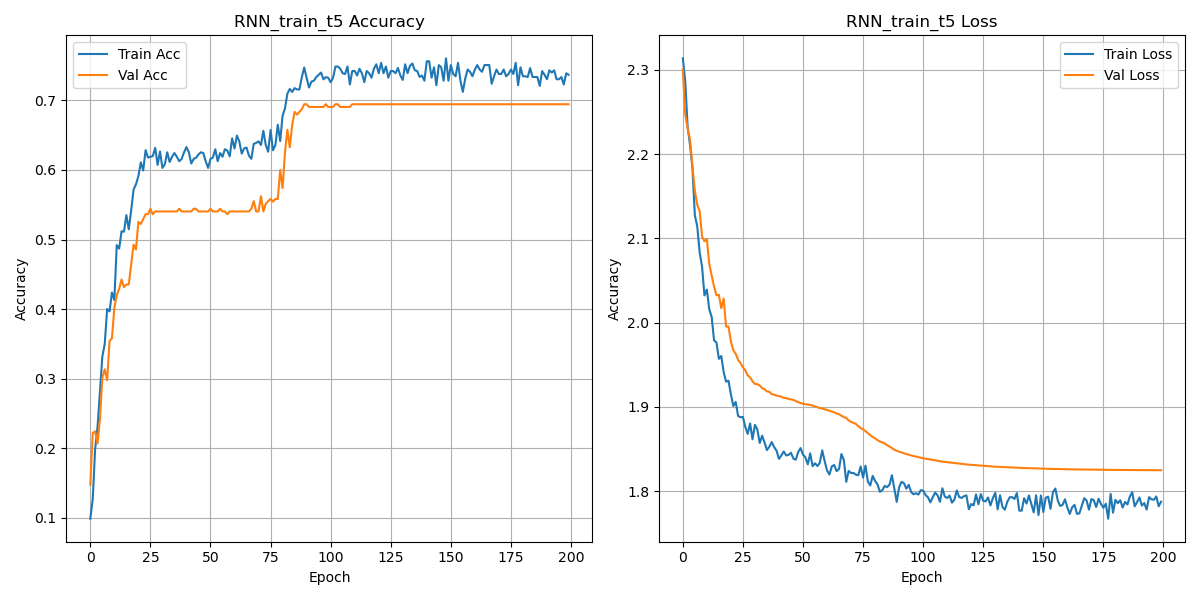
\includegraphics[width=\textwidth]{img/Part3/RNN_train_t5_fail.png}
    \caption{$T=5$ Fail Curve (with scheduler)}
  \end{subfigure}
  \caption{$T=5$ Curves}
  \label{fig:p3_t=5}
\end{figure}

\subsection{Result Analysis}

Through actual operations, I discovered a very strange situation: when training with $T=5$, 100\% accuracy can be achieved without the scheduler. After using the scheduler, this increase becomes very slow; on the contrary, in $ When T=20$, not using the scheduler will cause the model to degrade, but using it will keep the model 100\% accurate.

I compare the training success and "failure" curves together and guess some possible reasons.

\begin{itemize}
    \item First, analyze $T=5$. We know that \texttt{StepLR} can multiply the learning rate with $\gamma$ after a certain steps. This multiplication may cause an exponential explosion after several times, and the learning rate gradually drops to a very small value. Observing the normal curve without scheduler, we can find that the model reaches perfect accuracy after about 150 epochs. Therefore, if a scheduler is used, the model will not be able to effectively complete learning within a certain epoch, resulting in lower accuracy. But the learning rate still increased until the end
    
    \item {Second, for $T=20$, why does the accuracy become higher after using the scheduler? Observing the failure curve which without using the scheduler, we can find that the accuracy of the model reached a very high value at the beginning, but as the training continued, the accuracy experienced several sudden drops, and loss also appeared corresponding rising.
    
    My guess is that during the training process, it achieved very high accuracy at the beginning, but it did not perform a early stop, and gradient explosion occurred later. Although I used \texttt{clip\_grad\_norm\_()} correctly, it may be that the value of norm is too high, making it increasingly difficult to correct gradient explosion problem. Moreover, with the vanishing gradient problem caused by long dependencies of RNN, this makes correct learning more difficult.
    
    The use of the scheduler may have corrected this unexpected: after the epoch rises and before the gradient explosion occurs, the learning rate has been reduced to a very low value, simulating a early stop, so the impact of the gradient explosion has become very small, make it getting rid of significantly affect the entire model.
    }
\end{itemize}

Of course, the above is just guess which is not rigorous. Usually, in general, we will find that when the input length is low, RNN can eventually achieve a higher result, but once the input length becomes longer, its accuracy is very easy to decline. As the training continued, the model may seriously degrade. This can reflect a characteristic of RNN: the model's ability of memory is not very good. Once the input dependencies become longer, the problem of vanishing gradient occurs during training, which leads to poor learning results. The model will become very poor.

So in comparison, maybe using LSTM is a good choice.

\newpage

\begin{appendix}

\section{Extra Pictures}

\begin{figure}[!htbp]
  \centering
  \begin{subfigure}[b]{0.85\textwidth}
    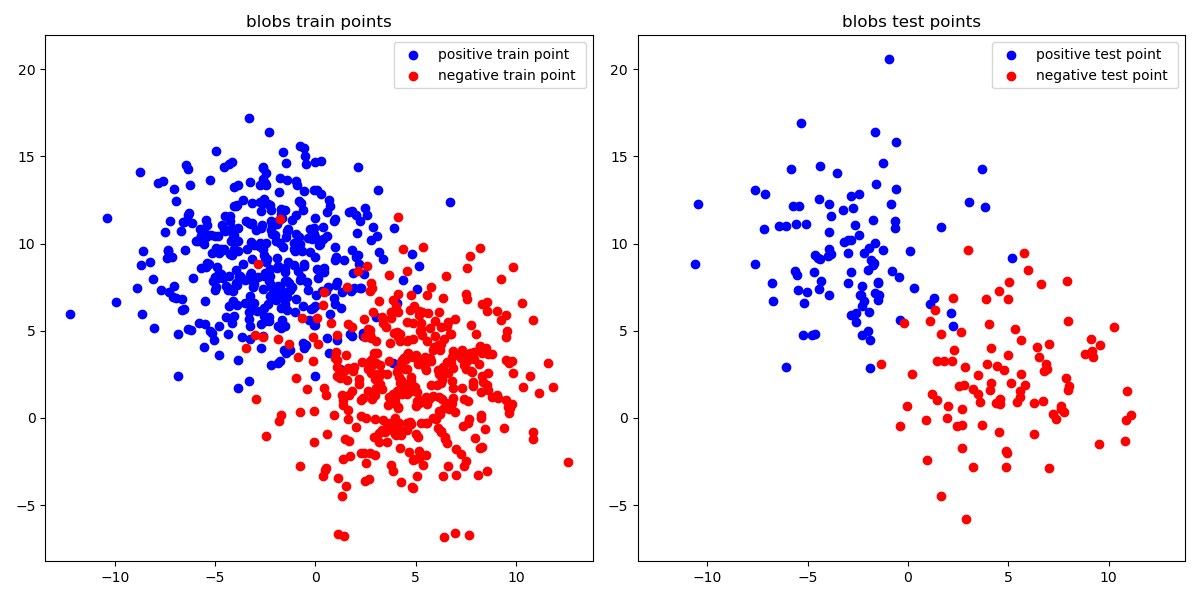
\includegraphics[width=\textwidth]{img/Part1/data_blobs.png}
    \caption{Moon Data}
  \end{subfigure}
  \begin{subfigure}[b]{0.90\textwidth}
    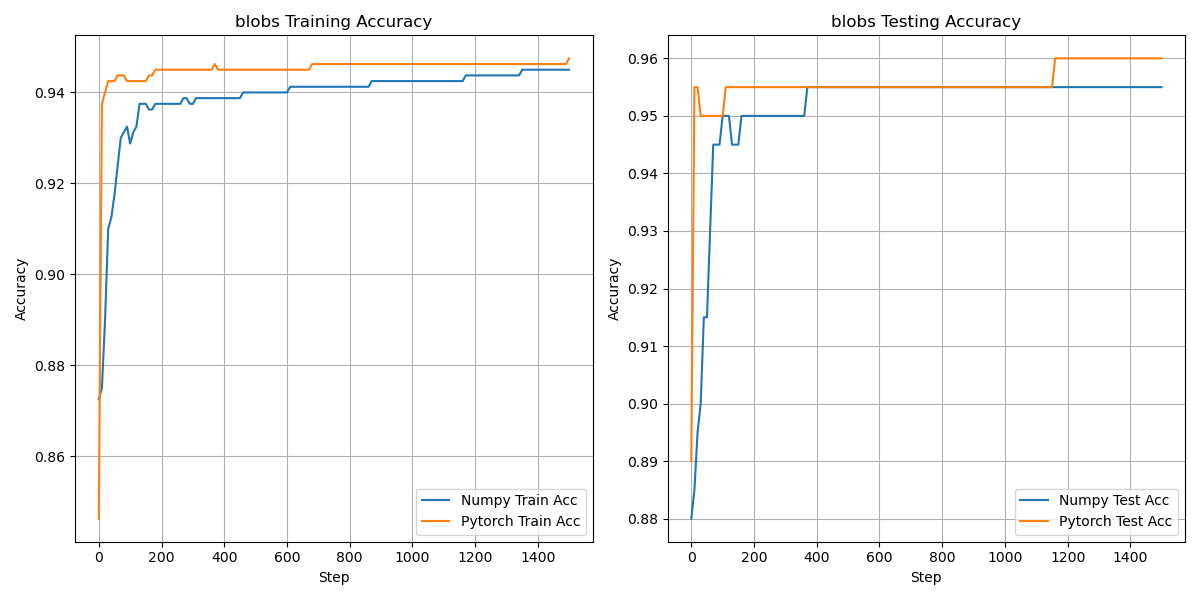
\includegraphics[width=\textwidth]{img/Part1/acc_blobs.png}
    \caption{Moon Accuracy}
  \end{subfigure}
  \begin{subfigure}[b]{0.90\textwidth}
    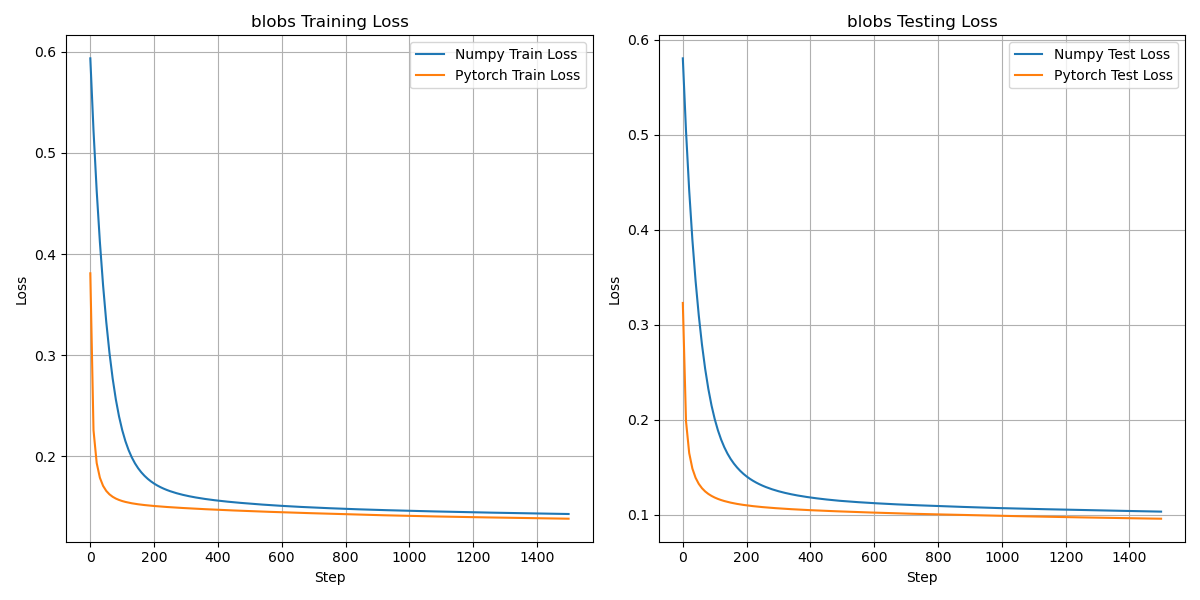
\includegraphics[width=\textwidth]{img/Part1/loss_blobs.png}
    \caption{Moon Loss}
  \end{subfigure}
  \caption{Moon numpy \& torch}
  \label{fig:p1t1_blobs}
\end{figure}

\begin{figure}[!htbp]
  \centering
  \begin{subfigure}[b]{0.85\textwidth}
    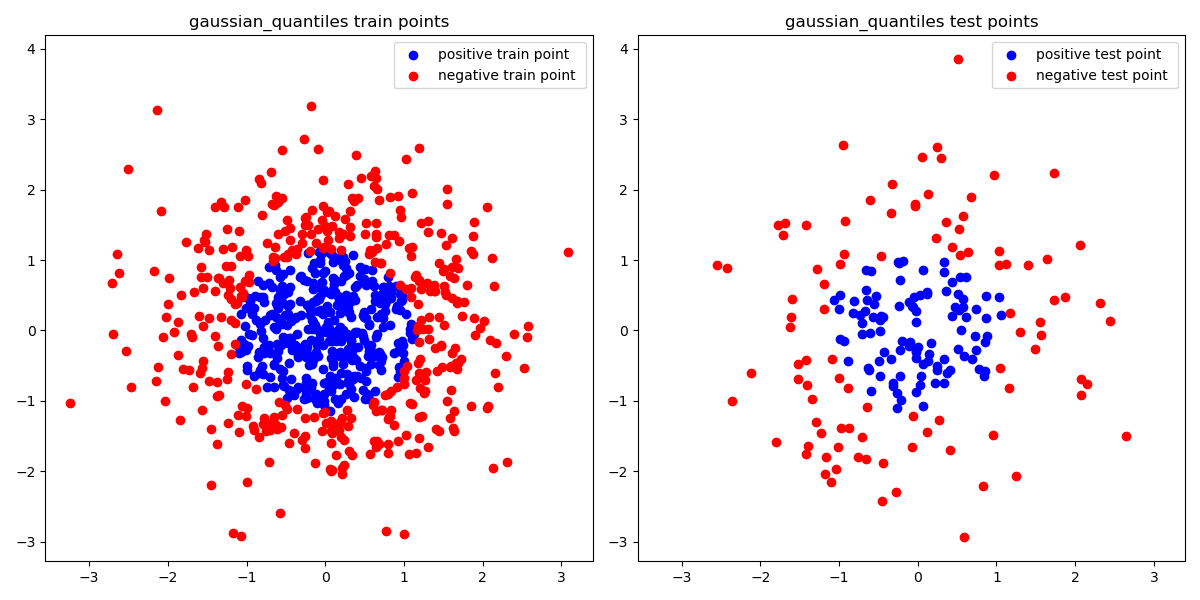
\includegraphics[width=\textwidth]{img/Part1/data_gaussian_quantiles.png}
    \caption{Gaussian Quantiles Data}
  \end{subfigure}
  \begin{subfigure}[b]{0.9\textwidth}
    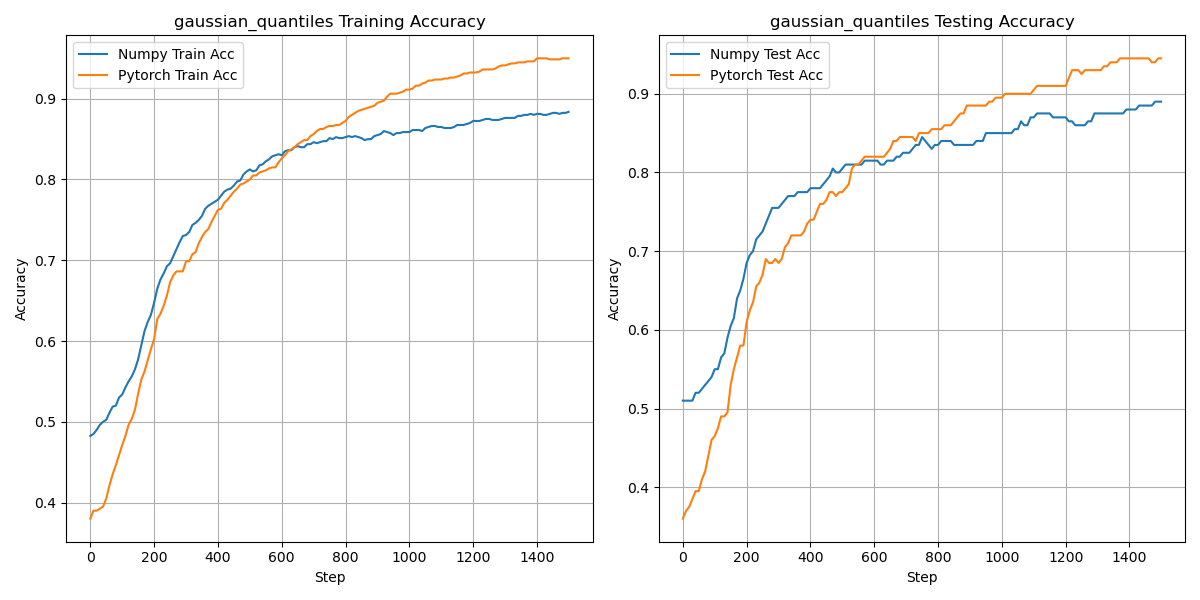
\includegraphics[width=\textwidth]{img/Part1/acc_gaussian_quantiles.png}
    \caption{Gaussian Quantiles Accuracy}
  \end{subfigure}
\begin{subfigure}[b]{0.9\textwidth}
    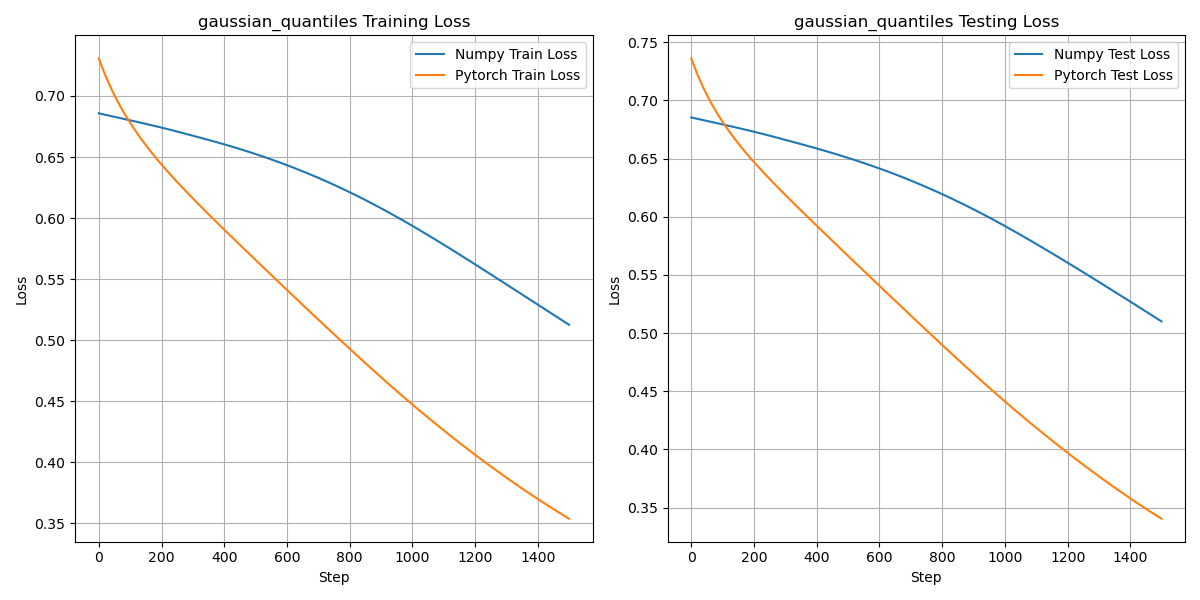
\includegraphics[width=\textwidth]{img/Part1/loss_gaussian_quantiles.png}
    \caption{Gaussian Quantiles Loss}
  \end{subfigure}
  \caption{Gaussian Quantiles numpy \& torch}
  \label{fig:p1t1_gaussian_quantiles}
\end{figure}

\begin{figure}[!htbp]
    \centering
    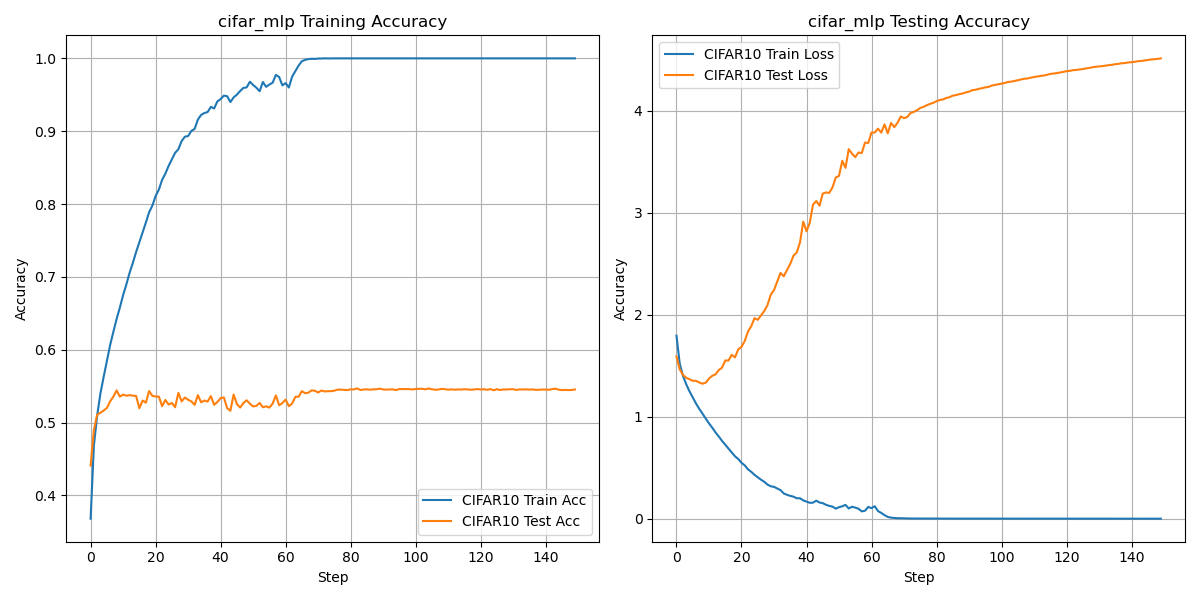
\includegraphics[width=1\textwidth]{img/Part1/cifar_mlp_b32_sgd.png}
    \caption{MLP CIFAR-10 Curve with SGD}
    \label{fig:p1t3_cifar_sgd}
\end{figure}

\begin{figure}[!htbp]
  \centering
  \begin{subfigure}[b]{1\textwidth}
    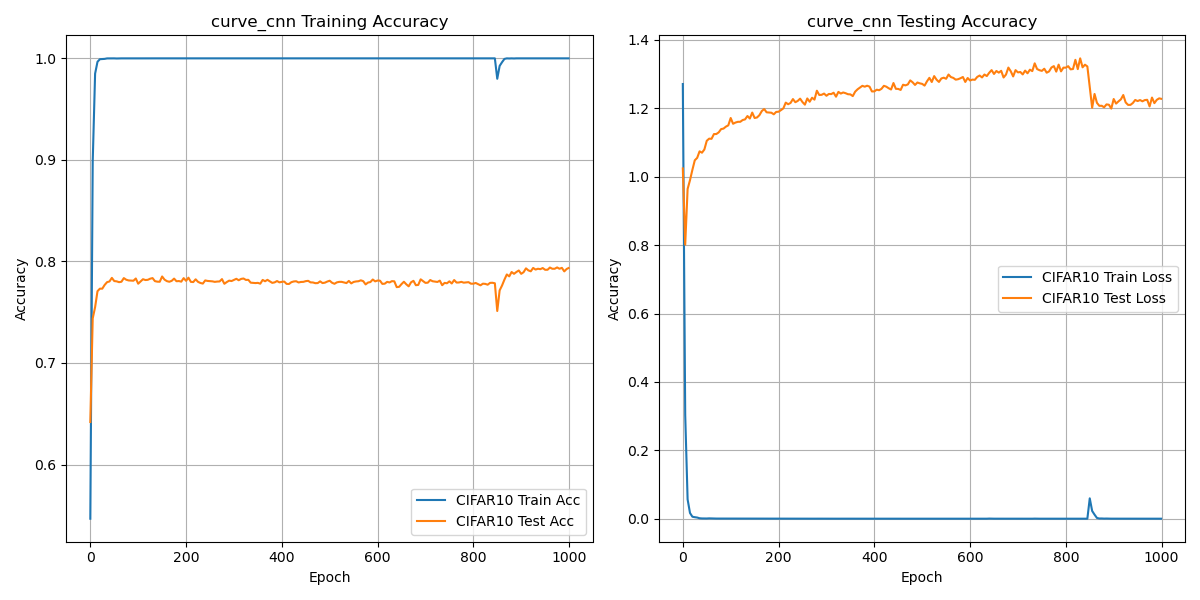
\includegraphics[width=\textwidth]{img/Part2/optimizer/curve_cnn_sgd.png}
    \caption{Accuracy and Loss}
  \end{subfigure}
  \begin{subfigure}[b]{1\textwidth}
    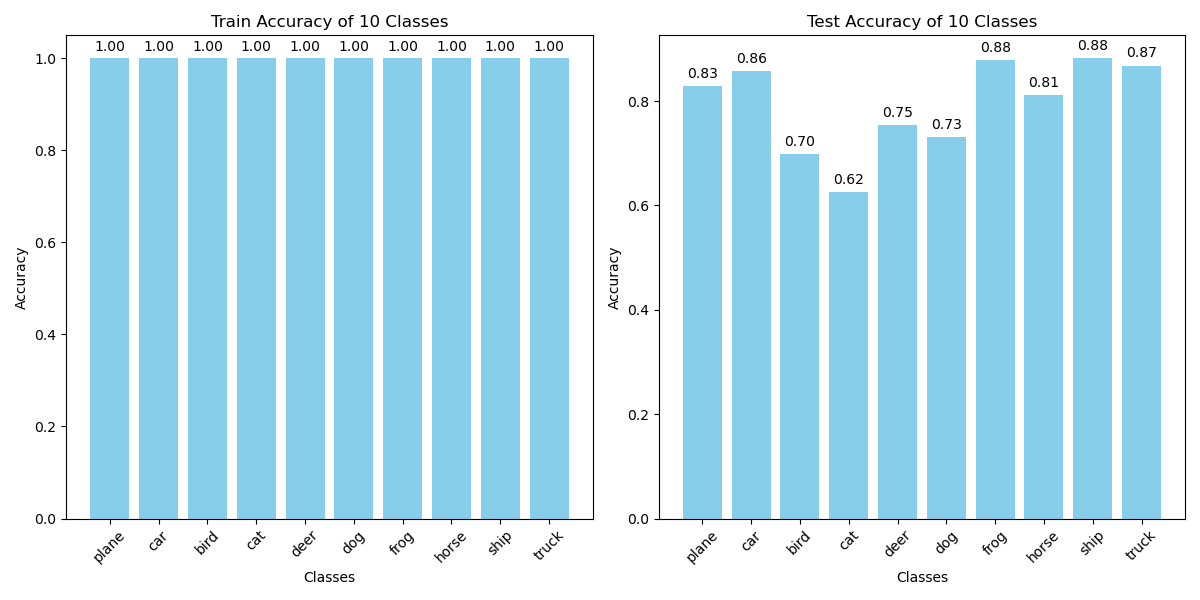
\includegraphics[width=\textwidth]{img/Part2/optimizer/acc_cnn_class_sgd.png}
    \caption{Class Accuracy}
  \end{subfigure}
  \caption{Optimizer SGD}
  \label{fig:p2_sgd}
\end{figure}

\begin{figure}[!htbp]
  \centering
  \begin{subfigure}[b]{1\textwidth}
    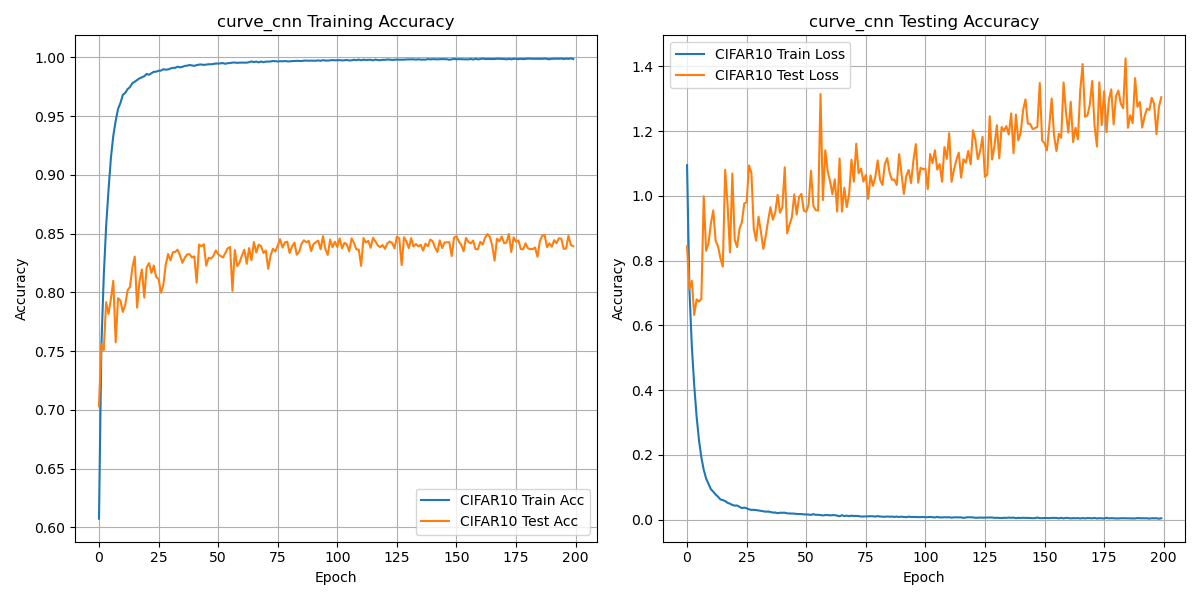
\includegraphics[width=\textwidth]{img/Part2/optimizer/curve_cnn_RMS.png}
    \caption{Accuracy and Loss}
  \end{subfigure}
  \begin{subfigure}[b]{1\textwidth}
    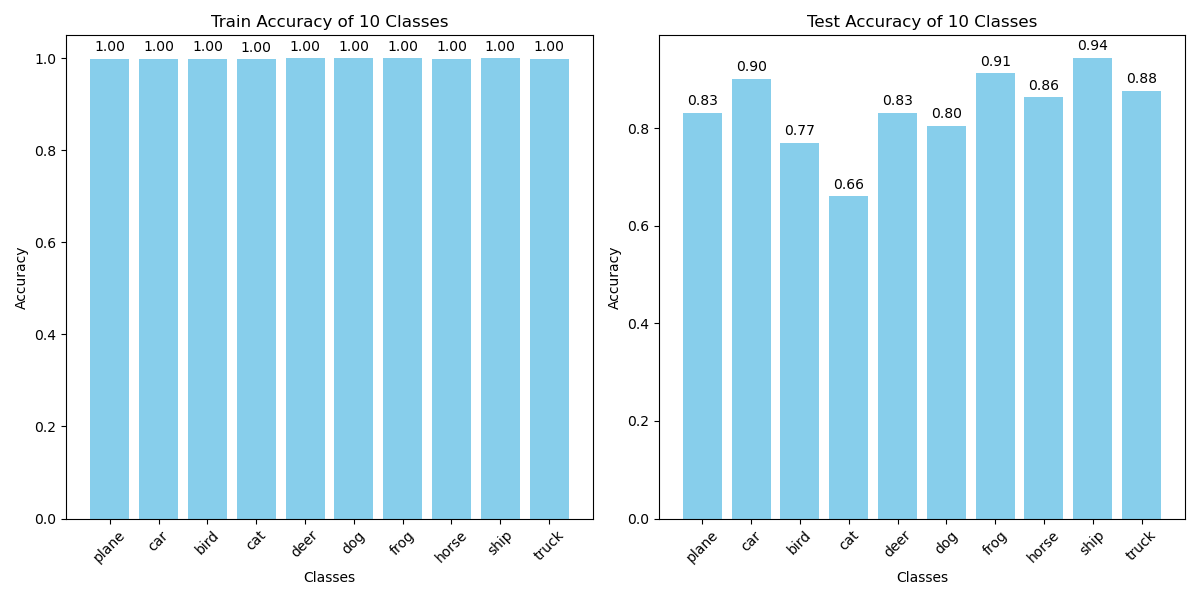
\includegraphics[width=\textwidth]{img/Part2/optimizer/acc_cnn_class_RMS.png}
    \caption{Class Accuracy}
  \end{subfigure}
  \caption{Optimizer RMS}
  \label{fig:p2_RMS}
\end{figure}

\begin{figure}[!htbp]
  \centering
  \begin{subfigure}[b]{1\textwidth}
    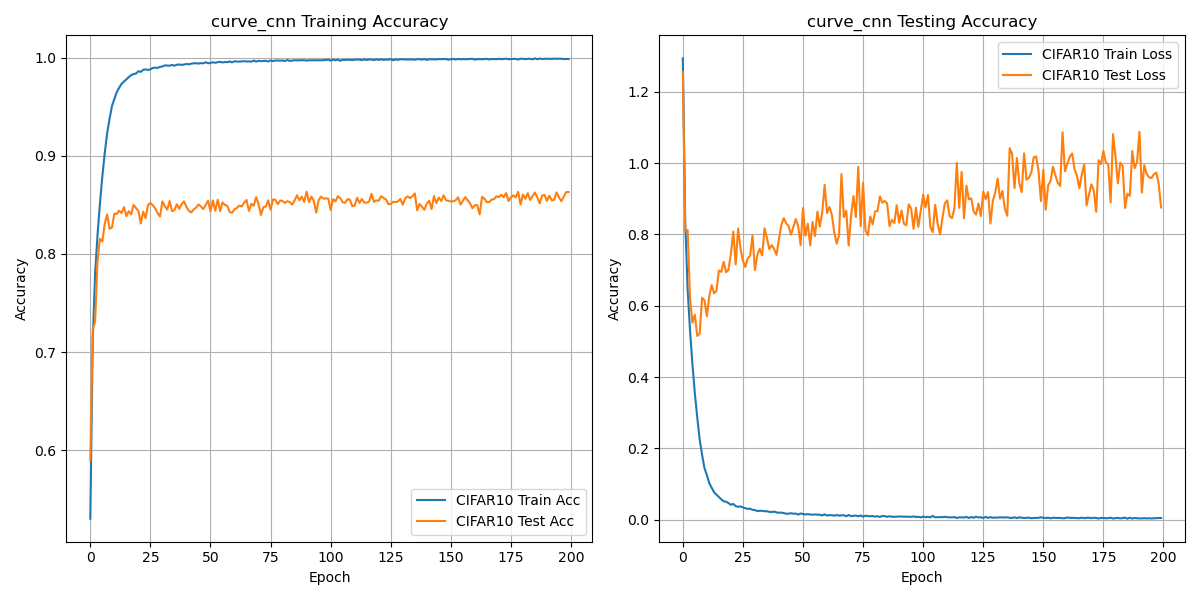
\includegraphics[width=\textwidth]{img/Part2/lr/curve_cnn_1e-3.png}
    \caption{Accuracy and Loss}
  \end{subfigure}
  \begin{subfigure}[b]{1\textwidth}
    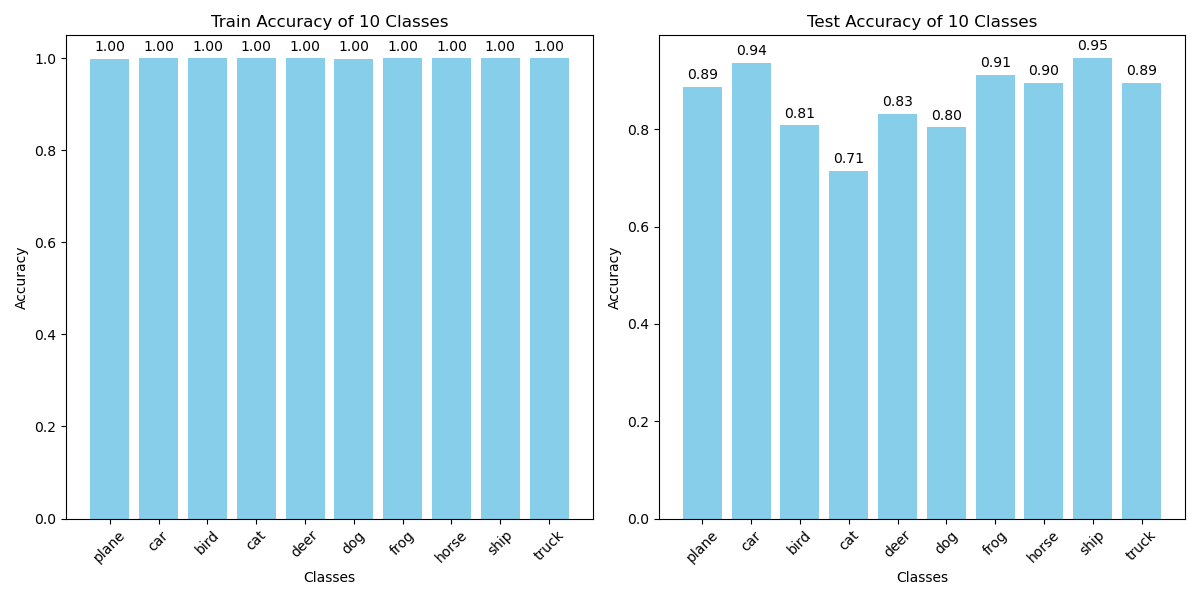
\includegraphics[width=\textwidth]{img/Part2/lr/acc_cnn_class_1e-3.png}
    \caption{Class Accuracy}
  \end{subfigure}
  \caption{Learning Rate $1\mathrm{e}^{-3}$}
  \label{fig:p2_lr_1e-3}
\end{figure}

\begin{figure}[!htbp]
  \centering
  \begin{subfigure}[b]{1\textwidth}
    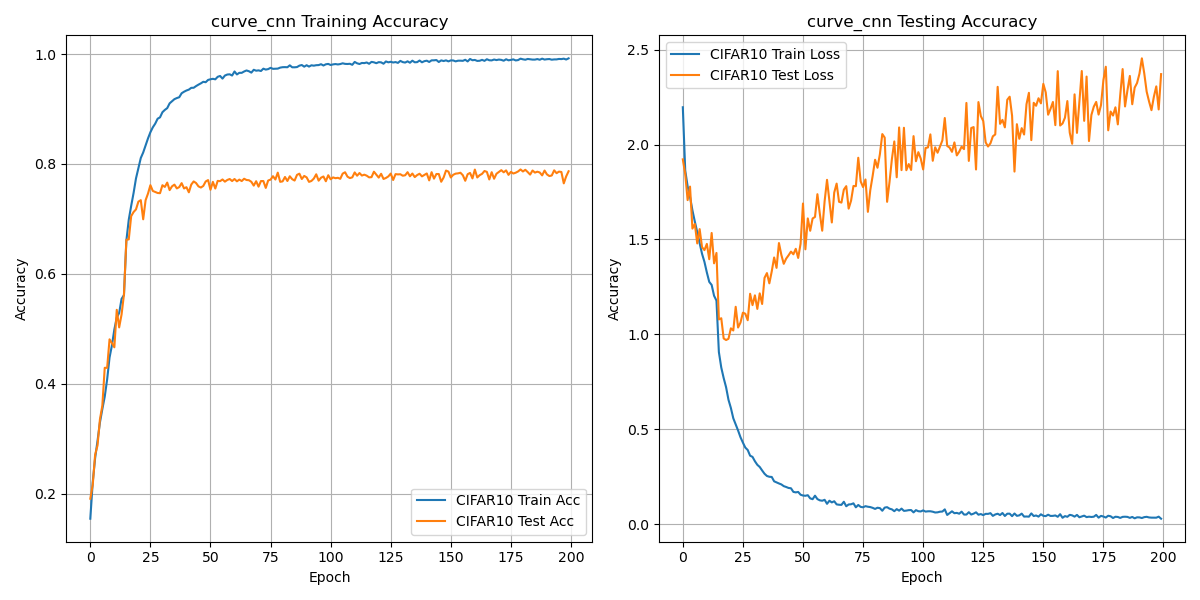
\includegraphics[width=\textwidth]{img/Part2/lr/curve_cnn_5e-2.png}
    \caption{Accuracy and Loss}
  \end{subfigure}
  \begin{subfigure}[b]{1\textwidth}
    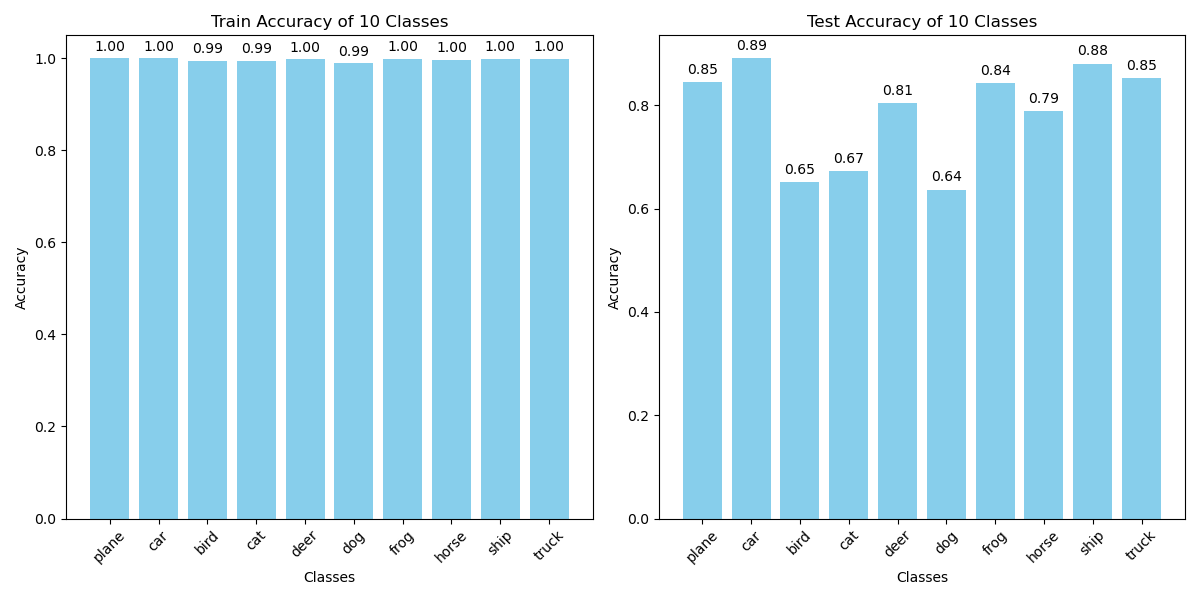
\includegraphics[width=\textwidth]{img/Part2/lr/acc_cnn_class_5e-2.png}
    \caption{Class Accuracy}
  \end{subfigure}
  \caption{Learning Rate $5\mathrm{e}^{-2}$}
  \label{fig:p2_lr_5e-2}
\end{figure}

\begin{figure}[!htbp]
  \centering
  \begin{subfigure}[b]{1\textwidth}
    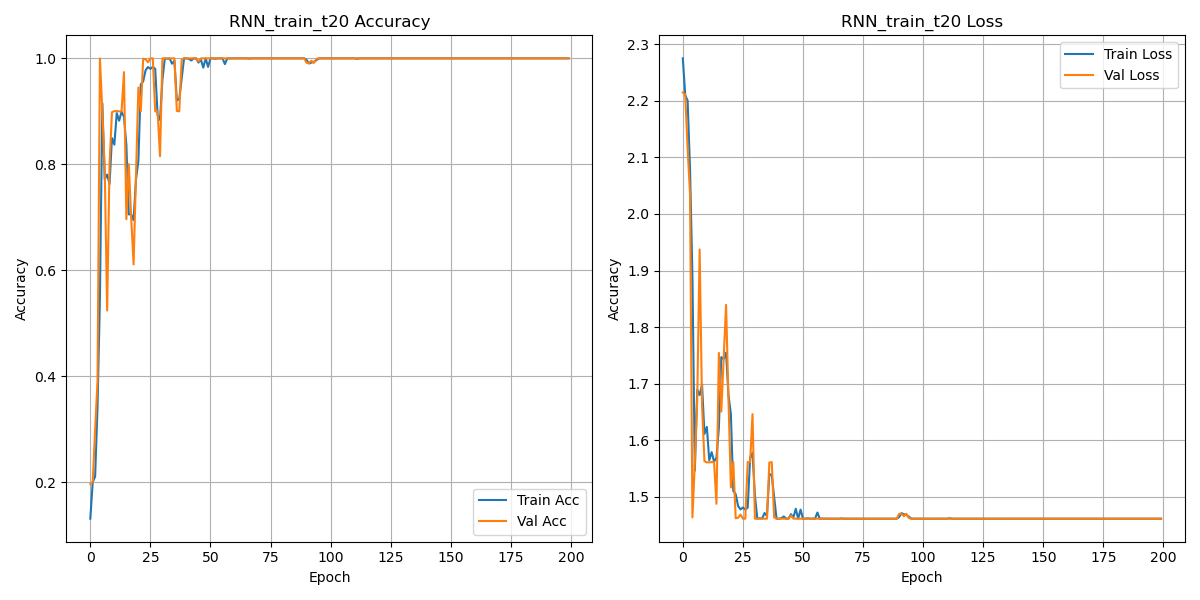
\includegraphics[width=\textwidth]{img/Part3/RNN_train_t20.png}
    \caption{$T=20$ Normal Curve (with scheduler)}
  \end{subfigure}
  \begin{subfigure}[b]{1\textwidth}
    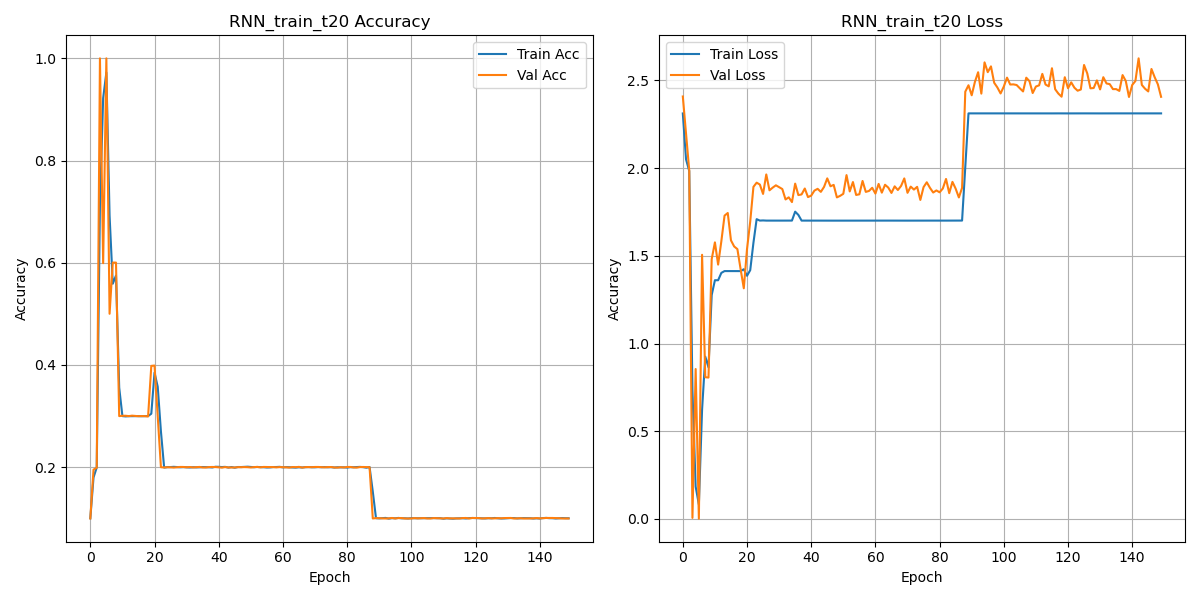
\includegraphics[width=\textwidth]{img/Part3/RNN_train_t20_fail.png}
    \caption{$T=20$ Fail Curve (without scheduler)}
  \end{subfigure}
  \caption{$T=20$ Curve}
  \label{fig:p3_t=20}
\end{figure}

\end{appendix}

\end{document}

